\documentclass[12pt]{report}
% \includeonly{chapters/specifica_dei_requisiti}
% xelatex documentazione.tex; makeglossaries documentazione; xelatex documentazione.tex 

\usepackage{geometry} % Impostazione dei margini e della rilegatura
\geometry{
	a4paper,
	left=1.5cm,    % margine sinistro
	right=1.5cm,   % Margine destro
	top=2.5cm,     % Margine superiore
	bottom=1.5cm   % Margine inferiore
} 

\usepackage{multicol}
\usepackage{tocloft}
\usepackage[]{lipsum}

\usepackage{hyperref} % permette agli hypertext di essere cliccabili
\hypersetup{
    pdftitle={Titolo PDF},
    pdfauthor={Autore PDF},
    colorlinks,
    linkcolor=black,
    citecolor=blue,
    filecolor=blue,
    urlcolor=blue
}

\usepackage{enumitem}
\setlist[itemize,enumerate]{
    topsep=0pt,
    itemsep=0pt,
    leftmargin=20pt
}

\usepackage{graphicx}

\usepackage{multirow}
\usepackage{float} 
\usepackage{tabularx}

\usepackage[table,xcdraw]{xcolor}

\usepackage{amssymb}
\usepackage{makecell}

\usepackage[italian]{babel}

\usepackage{glossaries}

\usepackage{tikz-uml}
\usetikzlibrary{positioning}

\usepackage{setspace}  % Per impostare l'interlinea
\setstretch{1.5} % Impostazioni per l'interlinea

\usepackage[explicit]{titlesec}
\titleformat{\chapter}[display]{\Huge\bfseries}{\centering #1}{0pt}{}
% \renewcommand{\thesection}{\arabic{section}}
\titlespacing*{\section}{0pt}{20pt}{5pt}
\titlespacing*{\subsection}{0pt}{15pt}{5pt}
\titlespacing*{\subsubsection}{0pt}{10pt}{5pt}

\usepackage{fancyhdr}
\pagestyle{fancy}
\fancypagestyle{plain}{%
  \renewcommand{\headrulewidth}{0pt}%
  \fancyhf{}%
}

\renewcommand{\chaptermark}[1]{\markboth{#1}{}}
\renewcommand{\sectionmark}[1]{\markright{#1}{}}
\fancyhead[L]{\leftmark}
\fancyhead[R]{\rightmark}
\newcommand{\sskip}{\smallskip \\ }
\newcommand{\meskip}{\medskip \\ }
\newcommand{\bskip }{\bigskip \\ }

\let\oldchapter\chapter
\renewcommand{\chapter}[1]{
    \newpage
    \begingroup%
    \let\clearpage\relax% Stop LaTeX from going to a new page
    % \vspace*{\fill}%
    \oldchapter{#1}
    % \vspace*{\fill}%
    \endgroup
    \thispagestyle{empty}
    % \newpage
}
% Comando personalizzato per stampare il glossario con il vecchio comportamento di \chapter
\newcommand{\printglossarywithchapter}{
    {\let\clearpage\relax\let\chapter\oldchapter\vspace{-15em}\chapter{Glossario}\printglossary}
}


\let\oldsection\section
\renewcommand{\section}[1]{
    % \newpage
    \oldsection{#1}
}

% \linespread{1.2} % imposta lo spazio tra le righe
\fontdimen2\font=0.5em % imposta spazio tra le parole
\renewcommand{\cellalign}{tl} % allinea le celle delle tabularx in alto a sinistra

\title{
    \includegraphics[width=120pt]{assets/logo_universita.pdf}\\
    Documentazione del software\\
    {\huge\textbf{DietiDeals24}}
}
\author{
    \begin{tabular}{lllll}
        Roberto Ingenito              &  & Simone Ingenito               &  & Lorenzo Sequino               \\
        \multicolumn{1}{c}{N86004077} &  & \multicolumn{1}{c}{N86004063} &  & \multicolumn{1}{c}{N86004367}
    \end{tabular}
    }
\date{Anno accademico 2023/2024}

% \setglossarystyle{listgroup}

\makeglossaries
% \newglossaryentry{latex}
% {
% 	name=latex,
% 	description={\lipsum[1]}
% }


\begin{document}

\maketitle

\newpage

\input{settings/table_of_contents.tex}

\newpage

\chapter{Introduzione}
\noindent DietiDeals24 è un'app mobile progettata per consentire agli utenti di creare e partecipare a diverse tipologie di aste in modo semplice e immediato. L'app supporta tre principali modalità di asta:

\begin{itemize}
    \item \textbf{Asta all'inglese}: Gli utenti fanno offerte incrementali, e l'oggetto va al miglior offerente.
    \item \textbf{Asta al ribasso}: L'asta parte da un prezzo massimo che diminuisce progressivamente fino a quando un utente decide di accettare il prezzo corrente.
    \item \textbf{Asta silenziosa}: Gli utenti inviano offerte in modo anonimo, e il vincitore viene determinato alla fine dell'asta senza che le offerte siano rese visibili durante il processo.
\end{itemize}

\noindent Gli utenti possono scegliere di partecipare come venditori, creando aste per i loro prodotti o servizi, oppure come acquirenti, facendo offerte per aggiudicarsi gli articoli in vendita. 
\include{chapters/analisi_dei_requisiti}
\chapter{Specifica dei requisiti}

\section{Modelli di dominio}
Quando si sviluppa un progetto software, è importante avere una chiara comprensione del sistema che si sta costruendo. Un modello di dominio aiuta a definire gli elementi principali del sistema, come interagiscono tra loro e come vengono rappresentati nel software.\sskip
Per strutturare il nostro modello di dominio, abbiamo adottato l'approccio "Three Object Type", che suddivide gli oggetti del sistema in tre categorie principali:
\begin{itemize}
	\item \textbf{Boundary}: Questi oggetti gestiscono l'interazione tra il sistema e gli attori esterni, come utenti o altri sistemi. Fungono da intermediari tra l'interfaccia utente e la logica interna dell'applicazione.
	\item \textbf{Control}: Questi oggetti implementano la logica di business e coordinano il flusso di dati tra gli oggetti Boundary e Entity. I Control mantengono separati gli aspetti di presentazione e quelli relativi ai dati, rendendo il sistema più facile da mantenere e migliorare.
	\item \textbf{Entity}: Questi oggetti sono utilizzati per modellare gli oggetti del mondo reale o concettuale che il sistema deve gestire e che devono essere persistenti, cioè mantenere il loro stato nel tempo.
\end{itemize}
\newpage

{ 	% NON RIMUOVERE LE PARENTESI GRAFFE CHE RACCHIUDONO GLI UML
	% blocco dei diagrammi uml in cui l'interlina è impostata a 1.2
	\setstretch{1.2}
	\subsection*{Registrazione e accesso}
	\begin{center}
	\scalebox{0.7}{
		\begin{tikzpicture}
			\umlclass[x=0, y=0, type=Boundary]{SignUpForm}{
				+ firstName: TextField\\
				+ lastName: TextField\\
				+ email: TextField\\
				+ password: TextField\\
				+ goToSignInPage: Button\\
				+ signUp: Button\\
			}{}

			\umlclass[x=10, y=0, type=Boundary]{SignInForm}{
				+ email: TextField\\
				+ password: TextField\\
				+ signIn: Button\\
				+ goToSignUpPage: Button\\
				+ signInWithGoogle: Button\\
			}{}
			\umlclass[x=5, y=-5, type=Boundary]{Feedback}{
				+ message: String \\
			}{}
			\umlclass[x=0, y=-9, type=Control]{SignUpController}{}{
				+ signUp(firstName, lastName, email, password)
			}
			\umlclass[x=10, y=-9, type=Control]{SignInController}{}{
				+ signIn(email, password)\\
				+ signInWithGoogle()
			}
			\umlclass[x=5, y=-15, type=Entity]{User}{
				+ firstName: String \\
				+ lastName: String \\
				+ email: String \\
				+ password: String \\
				+ bio: String \\
				+ webSiteLink: String \\
				+ profileImagePath: String \\
				+ socialLink: String[] \\
			}{}

			% Relationships
			\umlassoc[line width=2pt]{SignUpForm}{SignInForm}
			\umlassoc[line width=2pt]{SignUpForm}{SignUpController}
			\umlassoc[line width=2pt]{SignInForm}{SignInController}
			\umlassoc[line width=2pt]{SignUpController}{User}
			\umlassoc[line width=2pt]{SignInController}{User}
			\umlassoc[line width=2pt]{SignUpController}{Feedback}
			\umlassoc[line width=2pt]{SignInController}{Feedback}
		\end{tikzpicture}
	}
\end{center}
	\newpage

	\subsection*{Creazione asta silenziosa}
	\begin{center}
	\scalebox{0.7}{
		\begin{tikzpicture}
			\umlclass[type=Boundary, x=9, y=-4]{AuctionTypeCreationPage}{
				+ descendingAuctionButton: Button \\
				+ englishAuctionButton: Button \\
				+ silentAuctionButton: Button \\
			}{}

			\umlclass[type=Boundary, left=3cm of AuctionTypeCreationPage, yshift=1.5cm]{CreateDescendingAuction}{
			}{}

			\umlclass[type=Boundary, left=3cm of AuctionTypeCreationPage, yshift=-1.5cm]{CreateEnglishAuction}{
			}{}

			\umlclass[type=Boundary, right=2.5cm of AuctionTypeCreationPage, yshift=1cm]{NavBar}{
				+ createAuctionPageButton: Button\\
				+ homePageButton: Button\\
				+ auctionHistoryPageButton: Button\\
				+ profilePageButton: Button\\
			}{}

			\umlclass[type=Boundary, below=1cm of AuctionTypeCreationPage]{CreateSilentAuction}{
				+ loadImageButton: Button \\
				+ descriptionTextField: TextField \\
				+ categorySelect: Select \\
				+ dateTimePicker: DateTimePicker \\
				+ publishButton: Button \\
			}{}

			\umlclass[type=Control, below=1cm of CreateSilentAuction]{CreateAuctionController}{}{
				+ createSilentAuction(image, description, category, expirationDateTime) \\
				+ createDescendingAuction() \\
				+ createEnglishAuction()
			}

			\umlclass[type=Boundary, right=1cm of CreateAuctionController, yshift=4cm]{Feedback}{
				+ message: String
			}{}

			\umlclass[type=Entity, x=1, y=-19]{DescendingAuction}{
			}{}
			\umlclass[type=Entity, x=0, y=-22]{EnglishAuction}{
			}{}
			\umlclass[type=Entity, below=1cm of CreateAuctionController]{SilentAuction}{
				+ expirationDateTime: DateTime \\
			}{}

			\umlclass[type=Entity, below=1cm of SilentAuction]{Auction}{
				+ description: String \\
				+ imagePath: String \\
				+ category: String \\
			}{}

			\umlclass[below=1.5cm of Auction, type=Entity]{User}{
				+ firstName: String \\
				+ lastName: String \\
				+ email: String \\
				+ password: String \\
				+ bio: String \\
				+ webSiteLink: String \\
				+ profileImagePath: String \\
				+ socialLink: String[] \\
			}{}

			% Relationships
			\umlassoc{AuctionTypeCreationPage}{CreateDescendingAuction}
			\umlassoc{AuctionTypeCreationPage}{CreateEnglishAuction}
			\umlassoc{AuctionTypeCreationPage}{NavBar}
			\umlassoc{AuctionTypeCreationPage}{CreateSilentAuction}
			\umlassoc{CreateSilentAuction}{CreateAuctionController}
			\umlassoc{CreateAuctionController}{Feedback}
			\umlassoc{CreateAuctionController}{SilentAuction}
			\umlinherit{SilentAuction}{Auction}
			\umlinherit{EnglishAuction}{Auction}
			\umlinherit{DescendingAuction}{Auction}
			\umlassoc[mult2=1, mult1=0..*]{Auction}{User}
		\end{tikzpicture}
	}
\end{center}
	\newpage

	\subsection*{Creazione asta all'inglese}
	\begin{center}
	\scalebox{0.67}{
		\begin{tikzpicture}
			\umlclass[type=Boundary, x=9, y=-4]{CreateAuction}{
				+ descendingAuctionButton: Button \\
				+ englishAuctionButton: Button \\
				+ silentAuctionButton: Button \\
			}{}

			\umlclass[type=Boundary, x=0, y=-3]{CreateDescendingAuction}{
			}{}

			\umlclass[type=Boundary, x=3, y=0]{CreateSilentAuction}{
			}{}

			\umlclass[type=Boundary, x=14, y=0]{NavBar}{
				+ createAuctionButton: Button
			}{}

			\umlclass[type=Boundary, below=1cm of CreateAuction]{CreateEnglishAuction}{
				+ loadImageButton: Button \\
				+ descriptionTextField: TextField \\
				+ categorySelect: Select \\
				+ startingPriceTextField: TextField \\
				+ increaseThresholdTextField: TextField \\
				+ timerTextField: TextField \\
				+ publishButton: Button \\
			}{}

			\umlclass[type=Control, below=1cm of CreateEnglishAuction]{CreateAuctionController}{}{
				+ createEnglishAuction(image, description, category, startingPrice, increaseThreshold, timer) \\
				+ createDescendingAuction() \\
				+ createSilentAuction()
			}

			\umlclass[type=Boundary, right=1cm of CreateAuctionController, yshift=4cm]{Feedback}{
				+ message: String
			}{}

			\umlclass[type=Entity, below=1cm of CreateAuctionController]{EnglishAuction}{
				+ startingPrice: double \\
				+ increaseThreshold: double \\
				+ timer: int \\
			}{}

			\umlclass[type=Entity, below=1cm of EnglishAuction]{Auction}{
				+ description: String \\
				+ imagePath: String \\
				+ category: String \\
			}{}

			\umlclass[type=Entity, left=3cm of Auction, yshift=4cm]{DescendingAuction}{
			}{}
			\umlclass[type=Entity, left=5cm of Auction, yshift=1cm]{SilentAuction}{
			}{}

			\umlclass[below=1.5cm of Auction, type=Entity]{User}{
				+ firstName: String \\
				+ lastName: String \\
				+ email: String \\
				+ password: String \\
				+ bio: String \\
				+ webSiteLink: String \\
				+ profileImagePath: String \\
				+ socialLink: String[] \\
			}{}

			% Relationships
			\umlassoc{CreateAuction}{CreateDescendingAuction}
			\umlassoc{CreateAuction}{CreateSilentAuction}
			\umlassoc{CreateAuction}{NavBar}
			\umlassoc{CreateAuction}{CreateEnglishAuction}
			\umlassoc{CreateEnglishAuction}{CreateAuctionController}
			\umlassoc{CreateAuctionController}{Feedback}
			\umlassoc{CreateAuctionController}{EnglishAuction}
			\umlinherit{SilentAuction}{Auction}
			\umlinherit{EnglishAuction}{Auction}
			\umlinherit{DescendingAuction}{Auction}
			\umlassoc[mult2=1, mult1=0..*]{Auction}{User}
		\end{tikzpicture}
	}
\end{center}
	\newpage

	\subsection*{Creazione asta al ribasso}
	\begin{center}
	\scalebox{0.67}{
		\begin{tikzpicture}
			\umlclass[type=Boundary, x=9, y=0]{CreateAuction}{
				+ descendingAuctionButton: Button \\
				+ englishAuctionButton: Button \\
				+ silentAuctionButton: Button \\
			}{}

			\umlclass[type=Boundary, left=3cm of CreateAuction, yshift=1.5cm]{CreateEnglishAuction}{
			}{}
			
			\umlclass[type=Boundary, left=3cm of CreateAuction, yshift=-1.5cm]{CreateSilentAuction}{
			}{}

			\umlclass[type=Boundary, right=3cm of CreateAuction, yshift=1cm]{NavBar}{
				+ createAuctionButton: Button
			}{}

			\umlclass[type=Boundary, below=1cm of CreateAuction]{CreateDescendingAuction}{
				+ loadImageButton: Button \\
				+ descriptionTextField: TextField \\
				+ categorySelect: Select \\
				+ startingPriceTextField: TextField \\
				+ minimumPriceTextField: TextField \\
				+ decreaseAmountTextField: TextField \\
				+ decreaseTimeTextField: TextField \\
				+ publishButton: Button \\
			}{}

			\umlclass[type=Control, below=1cm of CreateDescendingAuction]{CreateAuctionController}{}{
				+ createDescendingAuction( image, description, category, \\
				\hspace{5cm}startingPrice, minimumPrice, \\
				\hspace{5cm}decreaseAmount, decreaseTime ) \\
				+ createEnglishAuction() \\
				+ createSilentAuction()
			}

			\umlclass[type=Boundary, right=1cm of CreateAuctionController, yshift=4cm]{Feedback}{
				+ message: String
			}{}

			\umlclass[type=Entity, below=1cm of CreateAuctionController]{DescendingAuction}{
				+ startingPrice: double \\
				+ minimumPrice: double \\
				+ decreaseAmount: double \\
				+ decreaseTime: int \\
			}{}

			\umlclass[type=Entity, below=1cm of DescendingAuction]{Auction}{
				+ description: String \\
				+ imagePath: String \\
				+ category: String \\
			}{}
			
			\umlclass[type=Entity, left=3cm of Auction, yshift=4cm]{EnglishAuction}{
			}{}
			\umlclass[type=Entity, left=5cm of Auction, yshift=1cm]{SilentAuction}{
			}{}

			\umlclass[below=1.5cm of Auction, type=Entity]{User}{
				+ firstName: String \\
				+ lastName: String \\
				+ email: String \\
				+ password: String \\
				+ bio: String \\
				+ webSiteLink: String \\
				+ profileImagePath: String \\
				+ socialLink: String[] \\
			}{}
			
			% Relationships
			\umlassoc{CreateAuction}{CreateEnglishAuction}
			\umlassoc{CreateAuction}{CreateSilentAuction}
			\umlassoc{CreateAuction}{NavBar}
			\umlassoc{CreateAuction}{CreateDescendingAuction}
			\umlassoc{CreateDescendingAuction}{CreateAuctionController}
			\umlassoc{CreateAuctionController}{Feedback}
			\umlassoc{CreateAuctionController}{DescendingAuction}
			\umlinherit{SilentAuction}{Auction}
			\umlinherit{DescendingAuction}{Auction}
			\umlinherit{EnglishAuction}{Auction}
			\umlassoc[mult2=1, mult1=0..*]{Auction}{User}
		\end{tikzpicture}
	}
\end{center}

	\newpage

	\subsection*{Puntare su un'asta silenziosa}
	\begin{center}
	\scalebox{0.7}{
		\begin{tikzpicture}
			\umlclass[type=Boundary]{AuctionDetailPage}{
			}{}

			\umlclass[above=3.5cm of AuctionDetailPage, xshift=4cm, type=Boundary]{EnglishAuctionDetailPage}{
			}{}

			\umlclass[above=3.5cm of AuctionDetailPage, xshift=-4cm, type=Boundary]{DescendingAuctionDetailPage}{
			}{}

			\umlclass[right=2cm of AuctionDetailPage, type=Boundary]{SilentAuctionDetailPage}{
				+ sellerProfileImage: Image \\
				+ sellerFullNameLabel: Text \\
				+ productImage: Image \\
				+ productDescriptionLabel: Text \\
				+ productExpirationLabel: Text \\
				+ offerTextField: TextField \\
				+ confirmOfferButton: Button \\
				+ showSellerProfilePageButton: Button \\
			}{}

			\umlclass[left=1.5cm of AuctionDetailPage, type=Boundary]{AuctionPage}{
				+ goToDetailPageButton: Button
			}{}

			\umlclass[above=1.5cm of AuctionPage, xshift=-4cm, type=Boundary]{HomePage}{
			}{}

			\umlclass[below=3cm of AuctionDetailPage, type=Control]{AuctionOfferController}{}{
				+ createSilentAuctionOffer(amount: double) \\
				+ createEnglishAuctionOffer() \\
				+ createDescendingAuctionOffer() \\
				+ showSellerProfilePage() \\
			}

			\umlclass[right=1.5cm of AuctionOfferController,type=Boundary]{Feedback}{
				+ message: String \\
			}{}

			\umlclass[below=1.5cm of AuctionOfferController, type=Entity]{SilentAuction}{
				+ expirationDateTime: DateTime
			}{}

			\umlclass[below=1.5cm of SilentAuction, type=Entity]{SilentAuctionOffer}{
				+ price: double \\
			}{}

			\umlclass[below=1.5cm of SilentAuctionOffer, type=Entity]{User}{
				+ firstName: String \\
				+ lastName: String \\
				+ email: String \\
				+ password: String \\
				+ bio: String \\
				+ webSiteLink: String \\
				+ profileImagePath: String \\
				+ socialLink: String[] \\
			}{}

			\umlclass[left=2.5cm of SilentAuction, type=Entity]{Auction}{
				+ description: String \\
				+ imagePath: String \\
				+ category: String \\
			}{}

			\umlclass[below=1.5cm of Auction, xshift=-2.5cm, type=Entity]{DescendingAuction}{
			}{}

			\umlclass[below=1.5cm of Auction, xshift=2.5cm, type=Entity]{EnglishAuction}{
			}{}



			\umlinherit{EnglishAuctionDetailPage}{AuctionDetailPage}
			\umlinherit{DescendingAuctionDetailPage}{AuctionDetailPage}
			\umlinherit{SilentAuctionDetailPage}{AuctionDetailPage}

			\umlinherit{DescendingAuction}{Auction}
			\umlinherit{EnglishAuction}{Auction}
			\umlinherit{SilentAuction}{Auction}

			\umlassoc[mult1=1, mult2=0..1]{User}{SilentAuctionOffer}
			\umlassoc[mult2=1, mult1=0..*]{SilentAuctionOffer}{SilentAuction}
			\umlassoc{SilentAuction}{AuctionOfferController}
			\umlassoc{AuctionOfferController}{Feedback}
			\umlassoc{AuctionOfferController}{AuctionDetailPage}
			\umlassoc{AuctionDetailPage}{AuctionPage}

			\umlaggreg{HomePage}{AuctionPage}


		\end{tikzpicture}
	}
\end{center}

	\newpage

	\subsection*{Puntare su un'asta all'inglese}
	\begin{center}
	\scalebox{0.7}{
		\begin{tikzpicture}
			\umlclass[type=Boundary]{AuctionDetailPage}{
			}{}

			\umlclass[above=3.5cm of AuctionDetailPage, xshift=4cm, type=Boundary]{SilentAuctionDetailPage}{
			}{}

			\umlclass[above=3.5cm of AuctionDetailPage, xshift=-4cm, type=Boundary]{DescendingAuctionDetailPage}{
			}{}

			\umlclass[right=2cm of AuctionDetailPage, type=Boundary]{EnglishAuctionDetailPage}{
				+ sellerProfileImage: Image \\
				+ sellerFullNameLabel: Text \\
				+ productImage: Image \\
				+ productDescriptionLabel: Text \\
				+ productExpirationLabel: Text \\
				+ lastOfferLabel: Text \\
				+ offerTextField: TextField \\
				+ confirmOfferButton: Button \\
				+ showSellerProfilePageButton: Button \\
			}{}

			\umlclass[left=1.5cm of AuctionDetailPage, type=Boundary]{AuctionPage}{
				+ goToDetailPageButton: Button
			}{}

			\umlclass[above=1.5cm of AuctionPage, xshift=-4cm, type=Boundary]{HomePage}{
			}{}

			\umlclass[below=3cm of AuctionDetailPage, type=Control]{AuctionOfferController}{}{
				+ createEnglishAuctionOffer(amount: double) \\
				+ createSilentAuctionOffer() \\
				+ createDescendingAuctionOffer() \\
				+ showSellerProfilePage() \\
			}

			\umlclass[right=1.5cm of AuctionOfferController,type=Boundary]{Feedback}{
				+ message: String \\
			}{}

			\umlclass[below=1.5cm of AuctionOfferController, type=Entity]{EnglishAuction}{
				+ startingPrice: double \\
				+ increaseThreshold: double \\
				+ timer: int \\
			}{}

			\umlclass[below=1.5cm of EnglishAuction, type=Entity]{EnglishAuctionOffer}{
				+ price: double \\
			}{}

			\umlclass[below=1.5cm of EnglishAuctionOffer, type=Entity]{User}{
				+ firstName: String \\
				+ lastName: String \\
				+ email: String \\
				+ password: String \\
				+ bio: String \\
				+ webSiteLink: String \\
				+ profileImagePath: String \\
				+ socialLink: String[] \\
			}{}

			\umlclass[left=2.5cm of EnglishAuction, type=Entity]{Auction}{
				+ description: String \\
				+ imagePath: String \\
				+ category: String \\
			}{}

			\umlclass[below=1.5cm of Auction, xshift=-2.5cm, type=Entity]{DescendingAuction}{
			}{}

			\umlclass[below=1.5cm of Auction, xshift=2.5cm, type=Entity]{SilentAuction}{
			}{}



			\umlinherit{SilentAuctionDetailPage}{AuctionDetailPage}
			\umlinherit{DescendingAuctionDetailPage}{AuctionDetailPage}
			\umlinherit{EnglishAuctionDetailPage}{AuctionDetailPage}

			\umlinherit{DescendingAuction}{Auction}
			\umlinherit{EnglishAuction}{Auction}
			\umlinherit{SilentAuction}{Auction}

			\umlassoc[mult1=1, mult2=0..1]{User}{EnglishAuctionOffer}
			\umlassoc[mult2=1, mult1=0..*]{EnglishAuctionOffer}{EnglishAuction}
			\umlassoc{EnglishAuction}{AuctionOfferController}
			\umlassoc{AuctionOfferController}{Feedback}
			\umlassoc{AuctionOfferController}{AuctionDetailPage}
			\umlassoc{AuctionDetailPage}{AuctionPage}

			\umlaggreg{HomePage}{AuctionPage}


		\end{tikzpicture}
	}
\end{center}

	\newpage

	\subsection*{Puntare su un'asta al ribasso}
	\begin{center}
	\scalebox{0.7}{
		\begin{tikzpicture}
			\umlclass[type=Boundary]{AuctionDetailPage}{
				+ sellerProfileImage: Image \\
				+ sellerFullNameLabel: Text \\
				+ productImage: Image \\
				+ productDescriptionLabel: Text \\
				+ confirmOfferButton: Button \\
				+ showSellerProfilePageButton: Button \\
			}{
				+ showSellerProfilePage() \\
			}

			\umlclass[above=2.5cm of AuctionDetailPage, xshift=4cm, type=Boundary]{SilentAuctionDetailPage}{
			}{}

			\umlclass[above=2.5cm of AuctionDetailPage, xshift=-4cm, type=Boundary]{EnglishAuctionDetailPage}{
			}{}

			\umlclass[right=2cm of AuctionDetailPage, type=Boundary]{DescendingAuctionDetailPage}{
				+ currentPriceLabel: Text \\
				+ decreaseTimerLabel: Text \\
				+ offerTextField: TextField \\
			}{}

			\umlclass[left=1.5cm of AuctionDetailPage, type=Boundary]{AuctionCard}{
				+ goToDetailPageButton: Button
			}{}

			\umlclass[above=1.5cm of AuctionCard, xshift=-2cm, type=Boundary]{HomePage}{
			}{}

			\umlclass[left=3cm of AuctionDetailPage, yshift=-4.5cm, type=Boundary]{SellerProfilePage}{
				fullNameLabel: Text \\
				profileImage: Image \\
				bio: Text \\
				webSiteLink: TextButton \\
				socialLinkList: TextButton[] \\
			}{}

			\umlclass[below=2cm of AuctionDetailPage, type=Control]{AuctionOfferController}{}{
				+ createDescendingAuctionOffer() \\
				+ createEnglishAuctionOffer() \\
				+ createSilentAuctionOffer() \\
			}

			\umlclass[right=1.5cm of AuctionOfferController,type=Boundary]{Feedback}{
				+ message: String \\
			}{}

			\umlclass[below=1.5cm of AuctionOfferController, type=Entity]{DescendingAuction}{
				+ startingPrice: double \\
				+ minimumPrice: double \\
				+ decreaseAmount: double \\
				+ decreaseTime: int \\
			}{}

			\umlclass[below=1.5cm of DescendingAuction, type=Entity]{DescendingAuctionOffer}{
				+ price: double \\
			}{}

			\umlclass[below=1.5cm of DescendingAuctionOffer, type=Entity]{User}{
				+ firstName: String \\
				+ lastName: String \\
				+ email: String \\
				+ password: String \\
				+ bio: String \\
				+ webSiteLink: String \\
				+ profileImagePath: String \\
				+ socialLink: String[] \\
			}{}

			\umlclass[left=2.5cm of DescendingAuction, type=Entity]{Auction}{
				+ description: String \\
				+ imagePath: String \\
				+ category: String \\
			}{}

			\umlclass[below=1.5cm of Auction, xshift=-2.5cm, type=Entity]{EnglishAuction}{
			}{}

			\umlclass[below=1.5cm of Auction, xshift=2.5cm, type=Entity]{SilentAuction}{
			}{}



			\umlinherit[line width=2pt]{SilentAuctionDetailPage}{AuctionDetailPage}
			\umlinherit[line width=2pt]{DescendingAuctionDetailPage}{AuctionDetailPage}
			\umlinherit[line width=2pt]{EnglishAuctionDetailPage}{AuctionDetailPage}

			\umlinherit[line width=2pt]{EnglishAuction}{Auction}
			\umlinherit[line width=2pt]{DescendingAuction}{Auction}
			\umlinherit[line width=2pt]{SilentAuction}{Auction}

			\umlassoc[line width=2pt, mult1=1, mult2=0..1]{User}{DescendingAuctionOffer}
			\umlassoc[line width=2pt, mult2=1, mult1=0..*]{DescendingAuctionOffer}{DescendingAuction}
			\umlassoc[line width=2pt]{DescendingAuction}{AuctionOfferController}
			\umlassoc[line width=2pt]{AuctionOfferController}{Feedback}
			\umlassoc[line width=2pt]{AuctionOfferController}{DescendingAuctionDetailPage}
			\umlassoc[line width=2pt]{AuctionDetailPage}{AuctionCard}
			\umlassoc[line width=2pt]{SellerProfilePage}{AuctionDetailPage}

			\umlaggreg[line width=2pt]{HomePage}{AuctionCard}
		\end{tikzpicture}
	}
\end{center}
	\newpage

	\subsection*{Storico aste (terminate)}
	\begin{center}
	\scalebox{0.68}{
		\begin{tikzpicture}
			\umlclass[x=0, y=0, type=Boundary]{AuctionsHistoryPage}{
				+ showPurchasedAuctionsPage: Button\\
				+ showCreatedAuctionsPage: Button\\
			}{}

			\umlclass[left=3cm of AuctionsHistoryPage, type=Boundary]{NavBar}{
				+ createAuctionPageButton: Button\\
				+ homePageButton: Button\\
				+ auctionHistoryPageButton: Button\\
				+ profilePageButton: Button\\
			}{}

			\umlclass[below=2cm of NavBar, xshift=-4cm, type=Boundary]{HomePage}{
			}{}

			\umlclass[below=1.5cm of AuctionsHistoryPage, xshift=-3.5cm, type=Boundary]{PurchasedAuctionsPage}{
			}{}

			\umlclass[below=1.5cm of AuctionsHistoryPage, xshift=3.5cm, type=Boundary]{CreatedAuctionsPage}{
			}{}

			\umlclass[below=5.3cm of AuctionsHistoryPage, type=Boundary]{AuctionCard}{
				+ image: Image \\
				+ category: Text \\
				+ description: Text \\
				+ isClosed: Text \\
				+ auctionDetailPageButton: Button \\
			}{}

			\umlclass[below=1cm of AuctionCard, type=Boundary]{AuctionDetailPage}{
				+ image: Image \\
				+ category: Text \\
				+ description: Text \\
			}{}

			\umlclass[left=2cm of AuctionDetailPage, type=Boundary]{PurchasedAuctionDetailPage}{
				+ offerAmount: Text \\
				+ sellerProfilePageButton: Button \\
			}{}

			\umlclass[right=2cm of AuctionDetailPage, type=Boundary]{CreatedAuctionDetailPage}{
				+ buyerFullName: Text \\
				+ offerAmount: Text \\
				+ buyerImage: Image \\
			}{}

			\umlclass[below=1cm of AuctionDetailPage, type=Control]{HistoryAuctionsController}{}{
				+ showSellerPage()
			}

			\umlclass[below=1cm of HistoryAuctionsController, type=Entity]{Auction}{
				+ description: String\\
				+ imagePath: String\\
				+ category: String\\
			}{}

			\umlclass[below=2cm of Auction, type=Entity]{User}{
				+ firstName: String \\
				+ lastName: String \\
				+ email: String \\
				+ password: String \\
				+ bio: String \\
				+ webSiteLink: String \\
				+ profileImagePath: String \\
				+ socialLink: String[] \\
			}{}




			% \umlinherit{SilentAuction}{Auction}
			% \umlassoc[mult1=1, mult2=0..1]{User}{DescendingAuctionOffer}
			% \umlaggreg{HomePage}{AuctionPage}
			\umlassoc{AuctionsHistoryPage}{NavBar}
			\umlassoc{NavBar}{HomePage}
			
			\umlcompo{AuctionsHistoryPage}{PurchasedAuctionsPage}
			\umlcompo{AuctionsHistoryPage}{CreatedAuctionsPage}

			\umlaggreg{PurchasedAuctionsPage}{AuctionCard}
			\umlaggreg{CreatedAuctionsPage}{AuctionCard}

			\umlassoc{AuctionCard}{AuctionDetailPage}
			\umlassoc{AuctionDetailPage}{HistoryAuctionsController}
			\umlassoc{HistoryAuctionsController}{Auction}
			\umlassoc[mult1=0..*, mult2=1]{Auction}{User}
			\umlinherit{CreatedAuctionDetailPage}{AuctionDetailPage}
			\umlinherit{PurchasedAuctionDetailPage}{AuctionDetailPage}

		\end{tikzpicture}
	}
\end{center}

	\newpage

	\subsection*{Asta silenziosa: accettazione di un'offerta}
	\begin{center}
	\scalebox{0.7}{
		\begin{tikzpicture}
			\umlclass[x=0, y=0, type=Boundary]{AuctionsHistoryPage}{
				+ showPurchasedAuctionsPage: Button\\
				+ showCreatedAuctionsPage: Button\\
			}{}

			\umlclass[right=3cm of AuctionsHistoryPage, type=Boundary]{NavBar}{
				+ createAuctionPageButton: Button\\
				+ homePageButton: Button\\
				+ auctionHistoryPageButton: Button\\
				+ profilePageButton: Button\\
			}{}

			\umlclass[below=2cm of NavBar, xshift=4cm, type=Boundary]{HomePage}{
			}{}

			\umlclass[below=1.5cm of AuctionsHistoryPage, xshift=-3.5cm, type=Boundary]{PurchasedAuctionsPage}{
			}{}

			\umlclass[below=1.5cm of AuctionsHistoryPage, xshift=3.5cm, type=Boundary]{CreatedAuctionsPage}{
			}{}

			\umlclass[below=5.3cm of AuctionsHistoryPage, type=Boundary]{AuctionCard}{
				+ image: Image \\
				+ category: Text \\
				+ description: Text \\
				+ isClosed: Text \\
				+ auctionDetailPageButton: Button \\
			}{}

			\umlclass[below=1cm of AuctionCard, type=Boundary]{AuctionDetailPage}{
				+ image: Image \\
				+ category: Text \\
				+ description: Text \\
			}{}

			\umlclass[right=2cm of AuctionDetailPage, type=Boundary]{SilentAcutionDetailPage}{
				+ buyerFullName: Text \\
				+ offerAmount: Text \\
				+ buyerImage: Image \\
			}{}

			\umlclass[right=3cm of SilentAcutionDetailPage, type=Boundary]{OfferContainer}{
				+ amountLabel: Text \\
				+ buyerFullNameLabel: Text \\
			}{}

			\umlclass[below=1cm of AuctionDetailPage, type=Control]{HistoryAuctionsController}{}{
				+ showSellerPage()\\
				+ acceptOffer(offer)\\
			}

			\umlclass[below=1cm of HistoryAuctionsController, type=Entity]{Auction}{
				+ description: String\\
				+ imagePath: String\\
				+ category: String\\
			}{}

			\umlclass[right=3cm of Auction, type=Entity]{Offer}{
				+ amount: double\\
			}{}

			\umlclass[right=3cm of Offer, type=Entity]{User}{
				+ firstName: String \\
				+ lastName: String \\
				+ email: String \\
				+ password: String \\
				+ bio: String \\
				+ webSiteLink: String \\
				+ profileImagePath: String \\
				+ socialLink: String[] \\
			}{}

			\umlassoc[line width=2pt]{AuctionsHistoryPage}{NavBar}
			\umlassoc[line width=2pt]{NavBar}{HomePage}
			
			\umlcompo[line width=2pt]{AuctionsHistoryPage}{PurchasedAuctionsPage}
			\umlcompo[line width=2pt]{AuctionsHistoryPage}{CreatedAuctionsPage}
			\umlcompo[line width=2pt, mult2=0..*, mult1=1]{SilentAcutionDetailPage}{OfferContainer}

			\umlaggreg[line width=2pt]{PurchasedAuctionsPage}{AuctionCard}
			\umlaggreg[line width=2pt]{CreatedAuctionsPage}{AuctionCard}

			\umlassoc[line width=2pt]{AuctionCard}{AuctionDetailPage}
			\umlassoc[line width=2pt]{AuctionDetailPage}{HistoryAuctionsController}
			\umlassoc[line width=2pt]{HistoryAuctionsController}{Auction}
			\umlassoc[line width=2pt, mult2=0..*, mult1=1]{Auction}{Offer}
			\umlassoc[line width=2pt, mult1=0..1, mult2=1]{Offer}{User}
			\umlinherit[line width=2pt]{SilentAcutionDetailPage}{AuctionDetailPage}

		\end{tikzpicture}
	}
\end{center}

	\newpage

	\subsection*{Modifica profilo}
	\begin{center}
	\scalebox{0.7}{
		\begin{tikzpicture}
			\umlclass[type=Boundary, x=0, y=0]{EditProfilePage}{
				+ firstNameTextField: TextField \\
				+ secondNameTextField: TextField \\
				+ bioTextField: TextField \\
				+ websiteLinkTextField: TextField \\
				+ geoPositionInput: Input \\
				+ updateInformationsButton: Button \\
				+ discardChangesButton: Button \\
				+ image: Image \\
				+ changeImageButton: Button \\
			}{}

			\umlclass[type=Boundary, above=2cm of EditProfilePage]{SocialLinkForm}{
				+ addNewSocialLinkButton: Button \\
			}{
				+ openSocialLinkBottomSheet() \\
			}

			\umlclass[type=Boundary, right=2cm of SocialLinkForm]{SocialLink}{
				+ socialLinkLabel: Text \\
				+ deleteSocialLinkButton: Button \\
			}{}

			\umlclass[type=Boundary, left=2cm of SocialLinkForm]{SocialLinkBottomSheet}{
				+ socialLinkTextField: TextField \\
				+ confirmButton: Button \\
			}{}

			\umlclass[type=Boundary, below=2cm of EditProfilePage]{ProfilePage}{
				+ firstNameLabel: Text \\
				+ lastNameLabel: Text \\
				+ bioLabel: Text \\
				+ websiteLinkButton: Button \\
				+ socialLinkButton: Button[] \\
				+ geoPositionLabel: Text \\
				+ editProfileButton: Button \\
				+ image: Image \\
			}{}

			\umlclass[type=Boundary, left=2cm of ProfilePage]{NavBar}{
				+ profilePageButton: Button\\
			}{}

			\umlclass[type=Control, below=2cm of ProfilePage]{ProfileController}{}{
				+ confirmInformationsUpdate() \\
			}

			\umlclass[type=Boundary, right=2cm of ProfileController]{Feedback}{
				+ message: Text \\
			}{}

			\umlclass[type=Entity, below=2cm of ProfileController]{User}{}{}

			% Relationships
			\umlcompo[line width=2pt]{SocialLinkForm}{SocialLink}
			\umlcompo[line width=2pt]{SocialLinkForm}{SocialLinkBottomSheet}
			\umlcompo[line width=2pt]{EditProfilePage}{SocialLinkForm}
			\umlaggreg[line width=2pt]{ProfilePage}{EditProfilePage}
			\umlassoc[line width=2pt]{ProfilePage}{NavBar}
			\umlassoc[line width=2pt]{ProfilePage}{ProfileController}
			\umlassoc[line width=2pt]{Feedback}{ProfileController}
			\umlassoc[line width=2pt]{User}{ProfileController}
		\end{tikzpicture}
	}
\end{center}

	\newpage

	\subsection*{Filtraggio e ricerca di un'asta}
	\begin{center}
	\scalebox{0.7}{
		\begin{tikzpicture}
			\umlclass[type=Boundary, x=0, y=0]{HomePage}{}{}

			\umlclass[type=Boundary, left=2cm of HomePage]{NavBar}{}{}

			\umlclass[type=Boundary, above=2cm of HomePage, xshift=-4cm]{AuctionCard}{}{}

			\umlclass[type=Boundary, above=2cm of HomePage, xshift=4cm]{SearchBar}{
				+ auctionDescriptionTextField: TextField \\
			}{}

			\umlclass[type=Boundary, right=2cm of HomePage]{CategoryButton}{
				+ categoryLabel: TextButton \\
			}{}

			\umlclass[type=Control, below=2cm of HomePage]{HomePageController}{}{
				+ filterAuctionsByDescription(patternText: String) \\
				+ filterAuctionsByCategory(category: String) \\
			}

			\umlclass[type=Boundary, right=2cm of HomePageController]{Feedback}{
				+ message: Text \\
			}{}

			\umlclass[type=Entity, below=2cm of HomePageController]{User}{}{}

			\umlclass[type=Entity, below=2cm of HomePageController, xshift=-6cm]{Auction}{
				+ category: String \\
				+ description: String \\
			}{}

			% Relationships
			\umlaggreg{HomePage}{CategoryButton}
			\umlaggreg{HomePage}{AuctionCard}
			\umlassoc{NavBar}{HomePage}
			\umlassoc{SearchBar}{HomePage}
			\umlassoc{HomePage}{HomePageController}
			\umlassoc{Feedback}{HomePageController}
			\umlassoc{User}{HomePageController}
			\umlassoc{Auction}{HomePageController}
		\end{tikzpicture}
	}
\end{center}

} % NON RIMUOVERE

\newpage
\section{Sequence diagram di due casi d'uso}
\subsection{Creazione asta all'inglese}
Questo Sequence Diagram descrive il processo di creazione di un'asta all'inglese. \\
L'attore principale è l'utente venditore che inizia il processo di creazione dell'asta inserendo i dati all'interno del form e cliccando il pulsante di creazione dell'asta.\\
A questo punto il sistema si occupa di gestire tutta la logica di creazione e di restituire un messaggio all'utente.\bskip
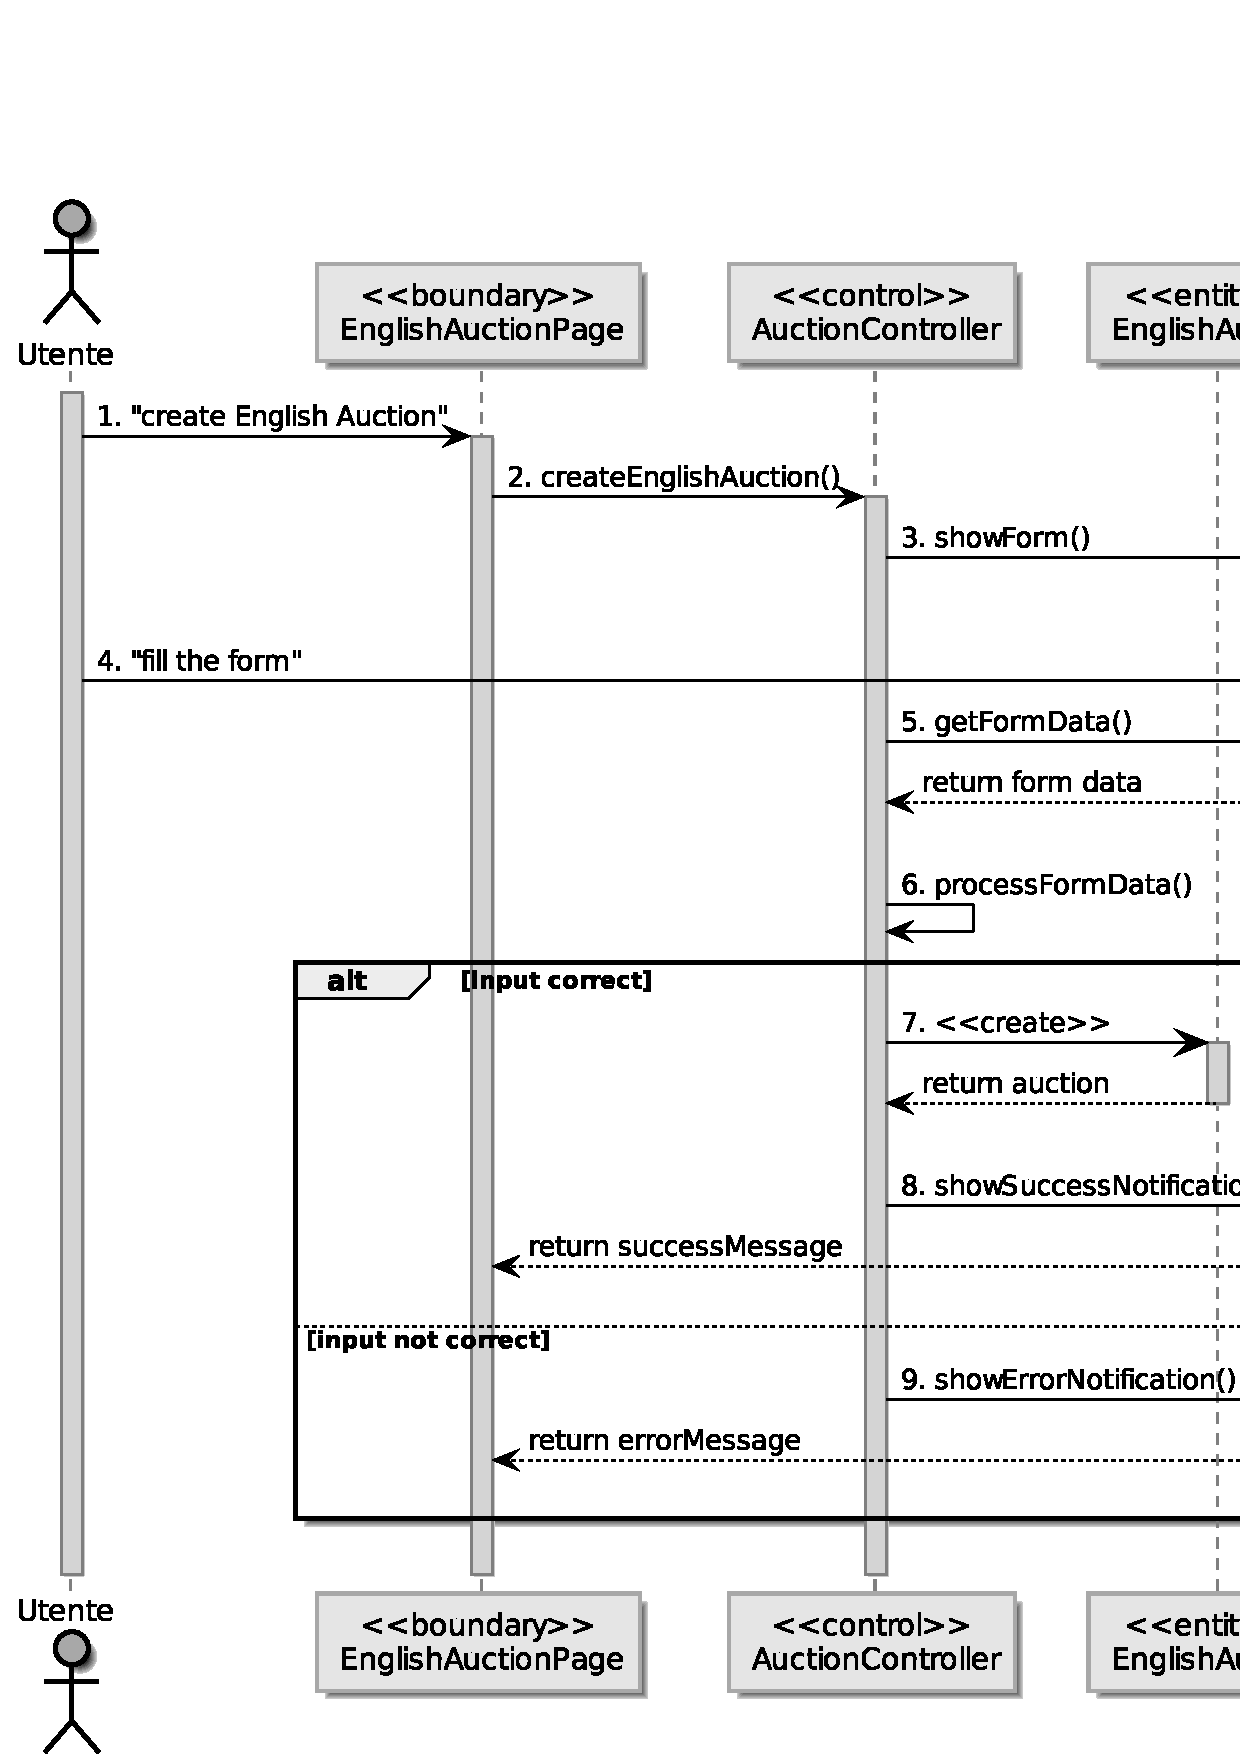
\includegraphics[width=\textwidth]{assets/sequence/creazione_asta_inglese.pdf}
\newpage

\subsection{Piazzare un'offerta su un'asta al ribasso}
Questo Sequence descrive il processo di creazione di un'offerta per un'asta al ribasso.\\
L'attore principale è l'utente acquirente che inizia il processo di creazione dell'offerta inserendo i dati all'interno del form e cliccando il pulsante di conferma.\\
Il sistema, dopo aver elaborato i dati, restituisce un messaggio all'utente.\bskip
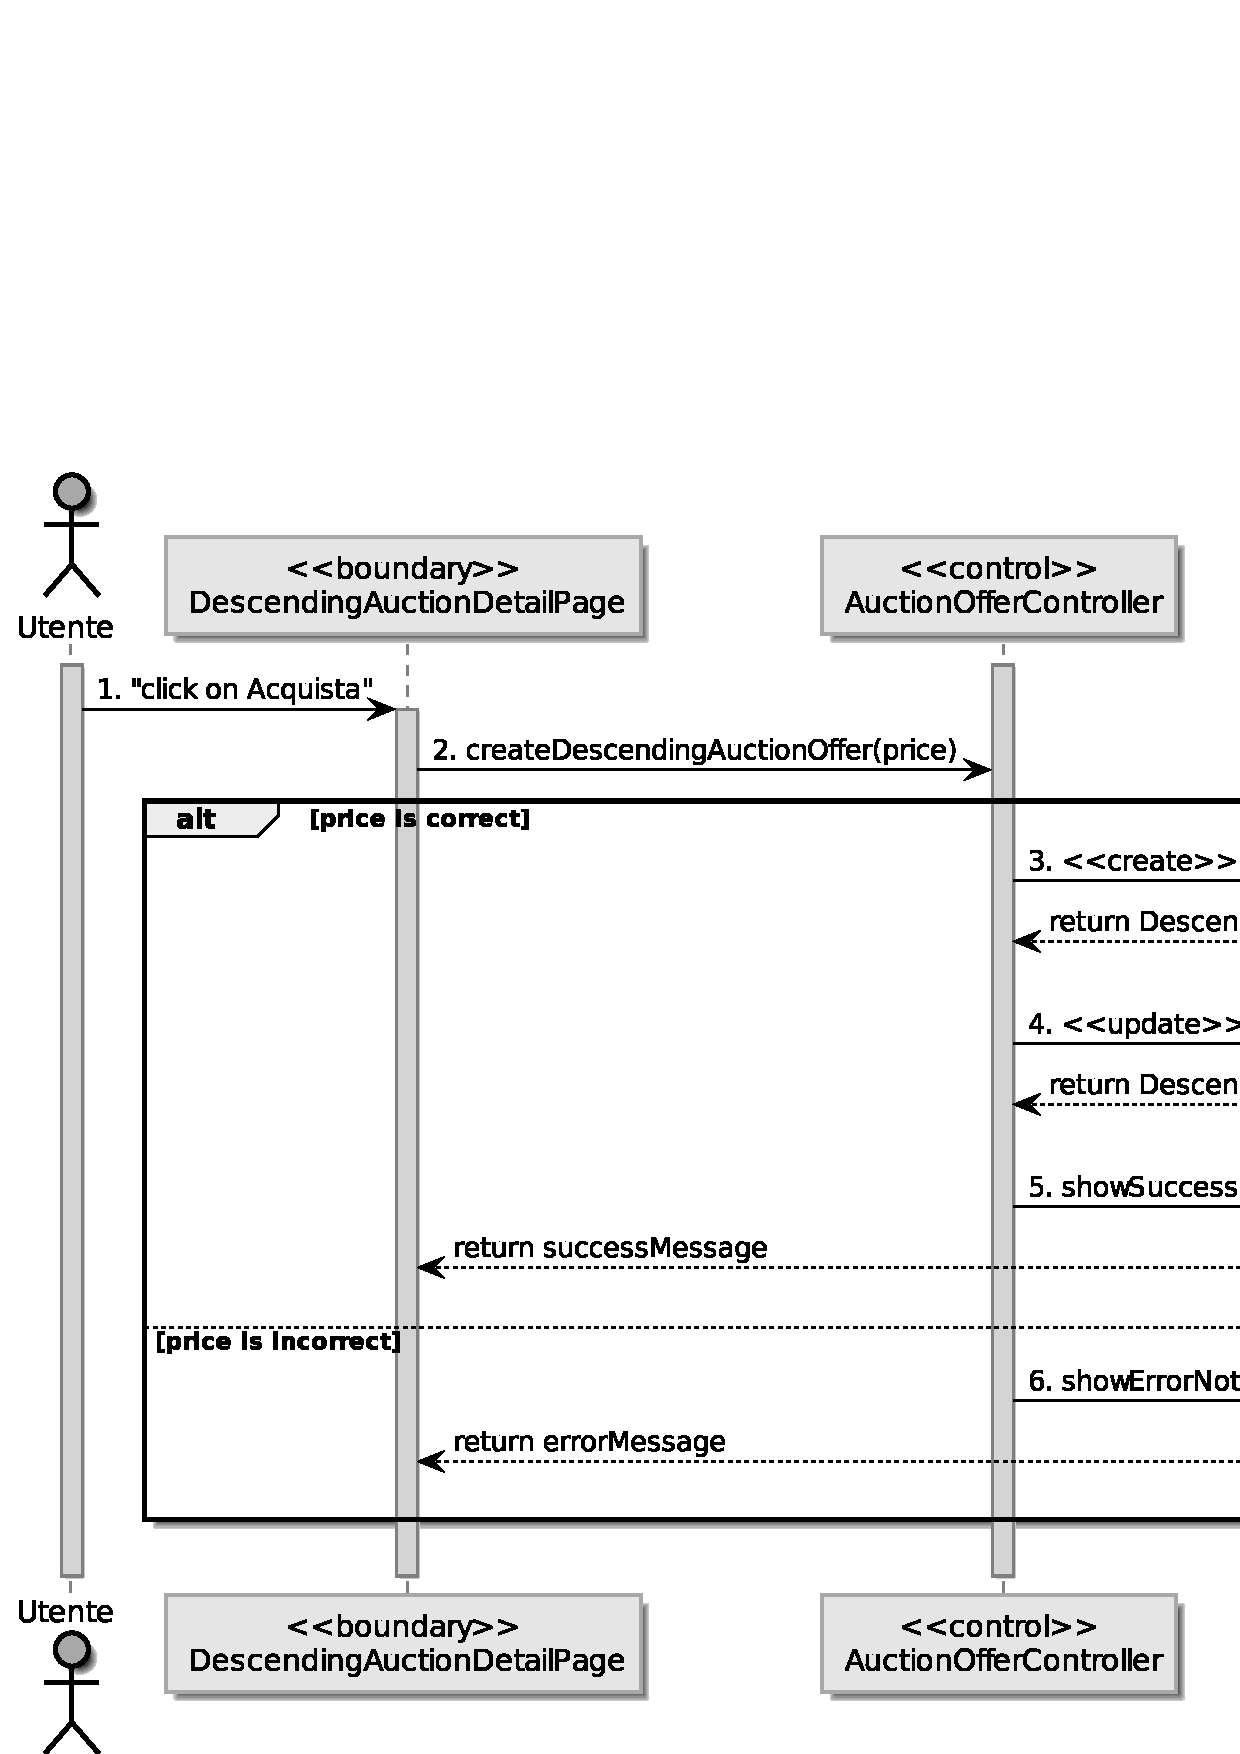
\includegraphics[width=\textwidth]{assets/sequence/piazzare_offerta_a_ribasso.pdf}
\newpage

\section{Progettazione degli Event-Based Statecharts}
Gli statecharts (o statechart diagrams) sono un tipo di diagramma utilizzato
per rappresentare il comportamento dinamico di un sistema attraverso
i suoi stati e le transizioni tra di essi.
\subsection{Creazione asta silenziosa}
Il seguente statechart descrive il comportamento del sistema durante la creazione di un'asta silenziosa.\\
Per prima cosa, l'utente si trova all'interno della schermata di selezione della tipologia d'asta da creare.
Dopo aver selezionato la tipologia d'asta corretta, il sistema passa alla pagina di creazione dell'asta, la quale contiene il form in cui inserire tutte le informazioni necessarie. Una volta che l'utente ha selezionato e inserito tutte le informazioni correttamente, l'asta viene creata e il sistema si aggiorna.\bskip
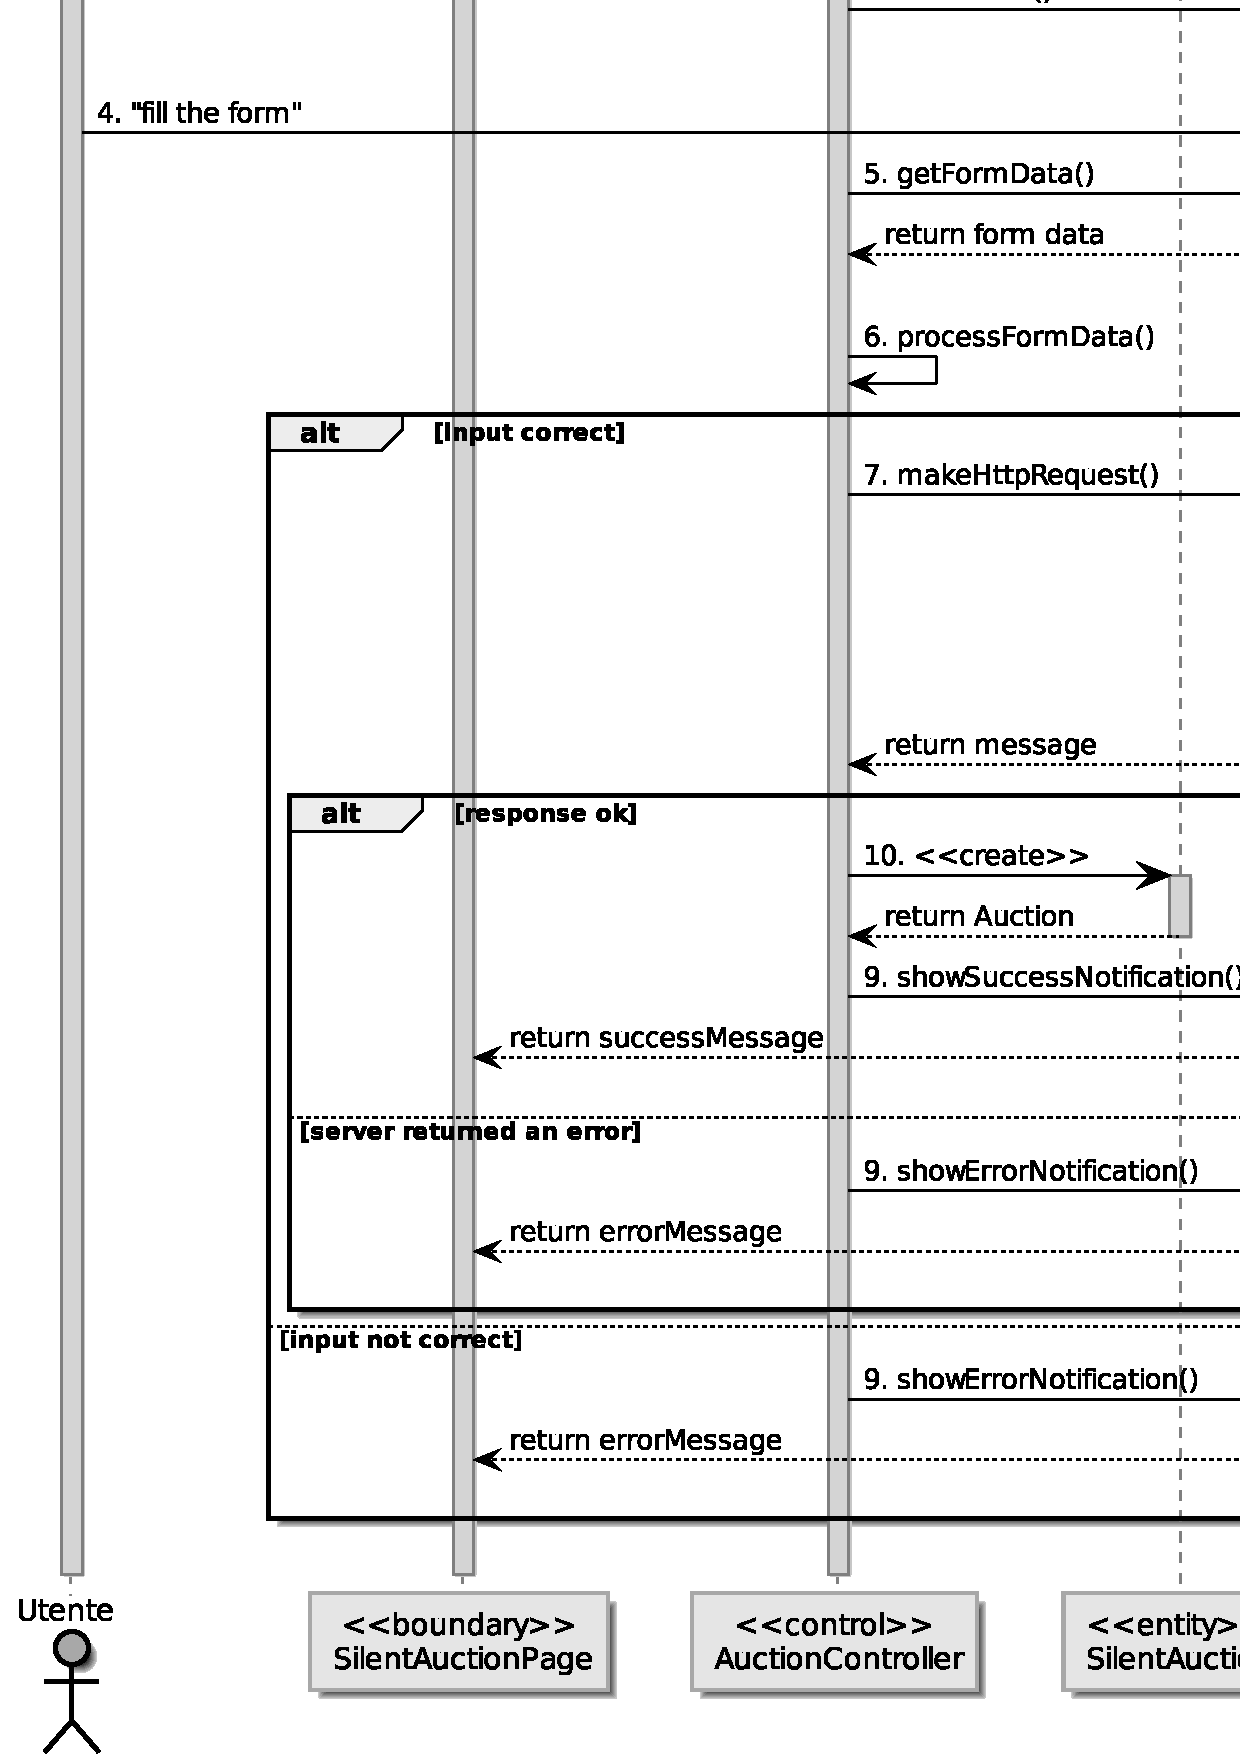
\includegraphics[width=\textwidth]{assets/state_charts/creazione_asta_silenziosa.pdf}
\newpage

\subsection{Offerta asta silenziosa}
Questo statechart descrive il comportamento del sistema durante la creazione di un'offerta per il tipo d'asta silenziosa.
Per prima cosa, l'utente seleziona l'asta cui desidera piazzare un'offerta.\\
Dopo aver effettuato la selezione il sistema passa alla schermata di dettaglio dell'asta, in cui è possibile inserire un'offerta.
Se l'offerta è corretta, il sistema si aggiorna correttamente.
\begin{center}
	\includegraphics[width=0.75\textwidth]{assets/state_charts/offerta_asta_silenziosa.pdf}
\end{center}
\newpage

\subsection{Aggiungi link social}
Questo statechart descrive il comportamento del sistema durante l'aggiunta di un link social. Nello specico, il sistema si trova in uno stato iniziale in cui è possibile visualizzare il profilo utente.
Dopodiche, il sistema passa nello stato di aggiornamento del profilo, in cui è possibile aggiungere un nuovo link social.
Dopo che il link è stato aggiunto, l'utente salva le modifiche e il sistema passa nello stato di profilo aggiornato.
\begin{center}
	\includegraphics[width=.75\textwidth]{assets/state_charts/aggiungi_link_social.pdf}
\end{center}
\newpage

\subsection{Visualizzare aste create}
Questo statechart descrive il comportamento del sistema quando l'utente vuole visualizzare lo storico delle aste create.
In particolare, il sistema può trovarsi in due sottostati diversi: schermata dello storico delle aste create, e la schermata dello storico delle aste acquistate.
Il sistema si ricorda dell'ultima schermata in cui si trovava precedentemente, che è di default la schermata delle aste create.
Da ognuna di queste due schermate è possibile passare all'altra.
\begin{center}
	\includegraphics[width=.75\textwidth]{assets/state_charts/visualizzare_aste_create.pdf}
\end{center}
\newpage
\chapter{Documento di design}
In questa sezione vengono illustrate le scelte architetturali e i design pattern adottati nel software.
Un design pattern è una soluzione generale e collaudata per risolvere problemi ricorrenti che si incontrano durante la progettazione di software.
Questi pattern possono migliorare la comprensione del codice, la manutenzione e la scalabilità di un'applicazione.

\bigskip\bigskip

\section{Architettura del Software}
L'architettura del software è suddivisa tra il client e il server, con il client sviluppato in Flutter e il server utilizzando AWS.

\subsection{Client}
L'applicazione client è sviluppata utilizzando Flutter, un framework open-source di Google per la creazione di applicazioni mobili nativamente compilate. Flutter consente di creare un'interfaccia utente ricca e reattiva, mantenendo un'alta performance sia su Android che iOS.\meskip
Il client sarà responsabile della visualizzazione dei dati e dell'interazione con l'utente.\\
La gestione dello stato sarà gestito tramite il pattern MVC (Model-View-Controller) integrato con i DAO (Data Access Object). 
Questo approccio separa la logica di business, la gestione dello stato e l'accesso ai dati, migliorando la manutenibilità e la testabilità del codice.

\subsection{Server}
Per la gestione del server, abbiamo scelto Amazon Web Services (AWS), una piattaforma cloud che offre un'ampia gamma di servizi, tra cui elaborazione, archiviazione, e database. 
Il server è stato implementato utilizzando un'istanza EC2, con un database gestito tramite RDS e la logica applicativa eseguita su un backend sviluppato in Express.


\subsection{Interazione tra Client e Server}
Il client invia richieste HTTP al backend seguento l'architettura REST. Il server riceve queste richieste, le elabora, e interagisce con il database per ottenere o aggiornare i dati.

Le risposte vengono restituite al client in formato JSON, garantendo così una facile integrazione e manipolazione dei dati all'interno dell'applicazione Flutter. 

La comunicazione tra client e server avviene attraverso richieste asincrone, che permettono al client di ottenere dati aggiornati in tempo reale senza interrompere l'esperienza dell'utente.



\section{Design pattern utilizzati}

\subsection{Model-View-Controller (MVC)}
Il pattern Model-View-Controller (MVC) è stato scelto per strutturare l'applicazione in modo da separare le responsabilità e facilitare la manutenzione del codice.

\begin{itemize}
	\item \textbf{Model}: Gestisce i dati dell'applicazione ed è responsabile della notifica alla View quando i dati cambiano. Questo permette alla View di aggiornarsi e riflettere le modifiche senza dover essere a conoscenza dei dettagli di come i dati sono gestiti.

	\item \textbf{View}: Si occupa della presentazione e dell'interfaccia utente. Mostra i dati agli utenti e aggiorna la visualizzazione in risposta alle modifiche del Model.

    \item \textbf{Controller}: Funziona da intermediario tra il Model e la View. Gestisce gli input degli utenti e aggiorna il Model e la View di conseguenza.
\end{itemize}

\subsection{Data Access Object (DAO)}
Il Data Access Object (DAO) è stato implementato per separare la logica di accesso ai dati dalla logica di business, semplificando la gestione e l'accesso ai dati.

\newpage
\section{Analisi delle scelte tecnologiche utilizzate}
\subsection{Client: Confronto con altre tecnologie}
La decisione di utilizzare flutter è stata presa dopo un'analisi delle opzioni disponibili, considerando vari fattori come la produttività, le prestazioni e la compatibilità.

\subsubsection{React Native}
\begin{itemize}
    \item \textbf{Prestazioni:} Flutter compila il codice direttamente in codice nativo, mentre React Native utilizza un ponte per comunicare tra JavaScript e codice nativo. Questo può portare a prestazioni superiori in Flutter.
    \item \textbf{Coerenza dell'UI:} Flutter utilizza un motore di rendering proprietario, che garantisce una coerenza visiva su tutte le piattaforme, mentre React Native si basa sui componenti nativi, il che può comportare variazioni tra iOS e Android.
\end{itemize}

\subsubsection{Sviluppo nativo (Java/Kotlin per Android, Swift per iOS)}
\begin{itemize}
    \item \textbf{Cross-Platform:} Flutter consente di scrivere un solo codice per entrambe le piattaforme, riducendo i tempi e i costi di sviluppo rispetto alla scrittura di codice separato.
    \item \textbf{Consistenza dell'Interfaccia:} Flutter offre un controllo totale sul rendering e sulla consistenza dell'interfaccia su entrambe le piattaforme.
    \item \textbf{Aggiornamenti e Manutenzione:} La manutenzione di una singola codebase è generalmente più semplice e meno costosa.
\end{itemize}

\subsection{Server}
\subsubsection{Amazon EC2}
\textit{Amazon Elastic Compute Cloud} (EC2) è il servizio di AWS che fornisce capacità di calcolo nel cloud. 
Tramite EC2, è possibile eseguire istanze di macchine virtuali configurabili in base alle esigenze del progetto, garantendo flessibilità e controllo totale sull'infrastruttura server.

Nel nostro caso, abbiamo implementato un server \textit{NodeJS} che esegue un backend \textit{express}.

\subsubsection{Amazon RDS}
\textit{Amazon Relational Database Service} (RDS) è il servizio gestito di AWS per database relazionali, che semplifica le attività di configurazione, gestione e scalabilità dei database. 

Nel nostro caso, abbiamo impiegato RDS con un database PostgreSQL.

\subsubsection{Express.js}
\textit{Express.js} è un framework per applicazioni web Node.js, utilizzato per sviluppare la logica applicativa del nostro backend. Ci ha permesso di implementare un'API RESTful in modo rapido ed efficiente, gestendo le richieste tra il client e il server e interfacciandosi con il database ospitato su RDS.
\chapter{Codice sorgente sviluppato}

\section{Strumento di Versioning}

\section{Report di qualità del codice}
\chapter{Report di Qualità del Codice}
La qualità del codice rappresenta un elemento fondamentale nello sviluppo software.
Un codice di alta qualità facilita la comprensione e la manutenzione da parte degli sviluppatori, riduce il numero di bug e vulnerabilità, aumentando la stabilità dell'applicazione.\par
Inoltre, un codice ben strutturato e pulito è essenziale per garantire la scalabilità del progetto. Permette di aggiungere nuove funzionalità senza compromettere le performance o l'affidabilità del sistema.

\section{SonarQube}
Per monitorare e migliorare la qualità del codice, è stato impiegato SonarQube. Questo permette di identificare potenziali bug, vulnerabilità e problemi tecnici, fornendo suggerimenti per ottimizzare il codice.
\begin{itemize}
    \item \textbf{Duplicazioni}: Le duplicazioni di codice possono portare a una maggiore complessità e difficoltà nella manutenzione. SonarQube rileva segmenti di codice duplicati e suggerisce di refattorizzarli per migliorare l'efficienza e ridurre il rischio di inconsistenze.

    \item \textbf{Bugs}: Rappresentano errori nel codice che possono causare comportamenti imprevisti o malfunzionamenti dell'applicazione.

    \item \textbf{Vulnerabilità}: Questi indici segnalano potenziali rischi di sicurezza presenti nel codice.
    
    \item \textbf{Code Smells}: Indicano aree del codice che, pur non essendo errori diretti, possono ridurre la leggibilità, la manutenibilità o la performance dell'applicazione.
\end{itemize}
\pagebreak
\subsection*{Duplicazioni}
Nel nostro progetto, il grafico delle duplicazioni di codice si è mantenuto costante nel tempo, nonostante l'incremento delle linee di codice complessive. Questo andamento positivo indica che, anche con la crescita del codice, siamo riusciti a gestire efficacemente la duplicazione, mantenendo un livello di duplicazione sotto controllo.\meskip
\includegraphics[width=\textwidth]{assets/sonarqube/duplication.png}

\subsection*{Errori}
Il grafico degli errori del nostro progetto presenta un andamento particolarmente positivo: inizia con un numero elevato di \textit{code smells} e mostra una costante diminuzione fino a raggiungere lo zero.\par
La diminuzione degli errori nel codice ha incrementato la stabilità dell'applicazione e riducendo i malfunzionamenti. Inoltre, ha facilitato la manutenzione e l'evoluzione del software, permettendo di aggiungere nuove funzionalità con maggiore sicurezza e minor rischio di introdurre nuovi bug.\meskip
\includegraphics[width=\textwidth]{assets/sonarqube/issues.png}
\chapter{Testing e Valutazione sul campo dell'Usabilità}

\section{Unit Testing}

All'interno del progetto lo Unit Testing è stato implementato seguendo la metodologia \textbf{Black Box.} Per l'implementazione di suddetti test è stato utilizzato il framework di testing nativo di Flutter che segue il modello xUnit come richiesto dal committente.

\subsection{checkEmailAndPassword}

Questo metodo ha la funzione di verificare che l'email e la password inserite in fase di registrazione rispettino i criteri di dominio per poter essere considerate valide.\meskip
Analizziamo quelle che sono le classi di equivalenza con le quali andremo a realizzare il testing:

\subsubsection*{EMAIL}

\begin{itemize}
	\item A1: L'email rispetta il pattern dell'espressione regolare (classe valida)
	\item A2: L'email non rispetta il pattern dell'espressione regolare (classe non valida)
\end{itemize}

\subsubsection*{PASSWORD}

\begin{itemize}
	\item B1: La password contiene da 0 a 7 caratteri (classe non valida)
	\item B2: La password contiene da 8 a 16 caratteri (classe valida)
	\item B3: La password contiene più di 16 caratteri (classe non valida)
\end{itemize}\medskip

\noindent
Utilizziamo come criterio di copertura R-WECT (Weak Robust Equivalence Class Testing) il quale ci garantisce un buon grado di copertura evitando però la scrittura di molti test case. In definitiva, un buon compromesso rispetto ai criteri SECT e WECT.\meskip
Testiamo ogni classe un'unica volta escludendo le combinazioni di classi non valide, otteniamo 3 test cases: A1 x B1, A2 x B2, A1 x B3.

\begin{lstlisting}[language=Dart]
group('Test checkEmailAndPassword con R-WECT', () {
  // Caso 1: Email valida, password troppo breve
  test('Email valida e password troppo breve (A1, B1)', () {
    expect(checkEmailAndPassword('test@example.com', 'short'), isFalse);
  });

  // Caso 2: Email non valida, password valida
  test('Email non valida e password valida (A2, B2)', () {
    expect(checkEmailAndPassword('invalid-email', 'validPass1'), isFalse);
  });

  // Caso 3: Email valida, password troppo lunga
  test('Email valida e password troppo lunga (A1, B3)', () {
    expect(checkEmailAndPassword('test@example.com', 'thisPasswordIsWayTooLong'), isFalse);
  });
});
    \end{lstlisting}
\newpage
\subsection{checkPriceDifference}

Questo metodo verifica che nella creazione dell'Asta al Ribasso, il prezzo minimo sia minore del prezzo iniziale e che siano entrambi maggiori di zero.\meskip
Analizziamo le classi di equivalenza:

\subsubsection*{minPrice}

\begin{itemize}
	\item A1: Il prezzo minimo è maggiore di zero e minore di startingPrice (classe valida)
	\item A2: Il prezzo minimo è minore di zero (classe non valida)
	\item A3: Il prezzo minimo è maggiore di zero e maggiore di startingPrice (classe non valida)
\end{itemize}

\subsubsection*{startingPrice}

\begin{itemize}
	\item B1: Il prezzo iniziale è maggiore di zero (classe valida)
	\item B2: Il prezzo iniziale è minore di zero (classe non valida)
\end{itemize}\medskip

\noindent
Potremmo utilizzare anche per questo metodo, il criterio di copertura R-WECT. Chiediamoci però, cosa succederebbe se il prezzo minimo fosse un valore molto vicino allo zero?

Consideriamo quindi una tecnica in questo caso migliore per effettuare il testing, il criterio \textbf{Boundary Values}, ossia il criterio dei valori limite. In questo caso, il numero di test case è pari a 9.\meskip
Per ogni parametro andiamo a testare: Il valore minimo, appena sopra il minimo, appena sotto al massimo, valore massimo e un test case con tutti i valori medi.

\begin{lstlisting}[language=Dart]
class PriceValidator {
  static bool validatePrices(double minPrice, double startingPrice) {
    if (minPrice <= 0 || startingPrice <= 0) return false;
    if (minPrice >= startingPrice) return false;
    return true;
  }
}

group('Test dei valori limite per checkPriceDifference', () {
  // Test con valori medi
  test('Test 1: Valori medi', () {
    expect(PriceValidator.validatePrices(50, 100), true);
  });

  // Test per minPrice (mantenendo startingPrice costante a 100)
  test('Test 2: minPrice al minimo', () {
    expect(PriceValidator.validatePrices(0.01, 100), true);
  });

  test('Test 3: minPrice appena sopra il minimo', () {
    expect(PriceValidator.validatePrices(0.02, 100), true);
  });

  test('Test 4: minPrice appena sotto il massimo', () {
    expect(PriceValidator.validatePrices(98, 100), true);
  });

  test('Test 5: minPrice al massimo', () {
    expect(PriceValidator.validatePrices(99, 100), true);
  });

  // Test per startingPrice (mantenendo minPrice costante a 50)
  test('Test 6: startingPrice al minimo', () {
    expect(PriceValidator.validatePrices(50, 50.01), true);
  });

  test('Test 7: startingPrice appena sopra il minimo', () {
    expect(PriceValidator.validatePrices(50, 50.02), true);
  });

  test('Test 8: startingPrice appena sotto il massimo', () {
    expect(PriceValidator.validatePrices(50, 999.99), true);
  });

  test('Test 9: startingPrice al massimo', () {
    expect(PriceValidator.validatePrices(50, 1000), true);
  });

  // Test aggiuntivi per casi non validi (per completezza)
  test('Test extra: minPrice negativo', () {
    expect(PriceValidator.validatePrices(-1, 100), false);
  });

  test('Test extra: startingPrice negativo', () {
    expect(PriceValidator.validatePrices(50, -1), false);
  });

  test('Test extra: minPrice maggiore di startingPrice', () {
    expect(PriceValidator.validatePrices(100, 50), false);
  });
});
    \end{lstlisting}
\newpage
\subsection{checkNewOfferPrice}

Questo metodo verifica che il nuovo importo per un'offerta in Asta all'Inglese sia maggiore di zero e maggiore dell'ultima offerta.\meskip
Analizziamo le classi di equivalenza:

\subsubsection*{newAmount}

\begin{itemize}
	\item A1: La nuova offerta è maggiore di zero e maggiore della precedente (classe valida)
	\item A2: La nuova offerta è minore di zero (classe non valida)
	\item A3: La nuova offerta è maggiore di zero ma minore della precedente (classe non valida)
\end{itemize}

\subsubsection*{previousAmount}

\begin{itemize}
	\item B1: La vecchia offerta è maggiore di zero (classe valida)
	\item B2: La vecchia offerta è minore di zero (classe non valida)
\end{itemize}\medskip

\noindent
Utilizziamo il criterio di copertura R-WECT sopra citato. Andiamo ad effettuare i seguenti test cases: A1 x B1, A2 x B1, A3 x B1, A1 x B2. Il numero di test cases necessari sarà 4.

\begin{lstlisting}[language=Dart]
class OfferValidator {
  static bool validateOffer(double newAmount, double previousAmount) {
    if (newAmount <= 0 || previousAmount <= 0) return false;
    if (newAmount <= previousAmount) return false;
    return true;
  }
}

group('R-WECT Tests for Bid Validation', () {
  // Test Case 1: A1 x B1 (tutte le classi valide)
  test('Test Case 1 (A1 x B1): Nuova offerta valida e vecchia offerta valida', () {
    // newAmount > previousAmount > 0
    expect(OfferValidator.validateOffer(100, 50), true);
  });

  // Test Case 2: A2 x B1 (newAmount negativo)
  test('Test Case 2 (A2 x B1): Nuova offerta negativa', () {
    // newAmount < 0, previousAmount > 0
    expect(OfferValidator.validateOffer(-10, 50), false);
  });

  // Test Case 3: A3 x B1 (newAmount minore del precedente)
  test('Test Case 3 (A3 x B1): Nuova offerta minore della precedente', () {
    // 0 < newAmount < previousAmount
    expect(OfferValidator.validateOffer(40, 50), false);
  });

  // Test Case 4: A1 x B2 (previousAmount negativo)
  test('Test Case 4 (A1 x B2): Vecchia offerta negativa', () {
    // newAmount > 0, previousAmount < 0
    expect(OfferValidator.validateOffer(100, -10), false);
  });
});
    \end{lstlisting}
\newpage
\subsection{checkBaseAndRaiseThreshold}

Questo metodo verifica che nella creazione dell'asta all'inglese la base d'asta e la soglia di rialzo siano entrambi maggiori di zero.\meskip
Analizziamo le classi di equivalenza:

\subsubsection*{basePrice}

\begin{itemize}
	\item A1: La base d'asta è minore di zero (classe non valida)
	\item A2: La base d'asta è maggiore di zero (classe valida)
\end{itemize}

\subsubsection*{increaseThreshold}

\begin{itemize}
	\item B1: La soglia di rialzo è minore di zero (classe non valida)
	\item B2: La soglia di rialzo è maggiore di zero (classe valida)
\end{itemize}\medskip

\noindent
Utilizziamo il criterio di copertura \textbf{Boundary Values}, ossia dei valori limiti. Il numero di test cases è sempre 9.

\begin{lstlisting}[language=Dart]
class AuctionValidator {
  static bool validateAuctionParameters(double basePrice, double increaseThreshold) {
    if (basePrice <= 0 || increaseThreshold <= 0) return false;
    return true;
  }
}

group('Boundary Value Analysis Tests for Auction Parameters', () {
  // Test con valori nominali (il +1)
  test('Test 1: Valori nominali', () {
    expect(AuctionValidator.validateAuctionParameters(100, 10), true);
  });

  // Test per basePrice (primi 4 test, mantenendo increaseThreshold costante)
  test('Test 2: basePrice al minimo', () {
    expect(AuctionValidator.validateAuctionParameters(0.01, 10), true);
  });

  test('Test 3: basePrice appena sopra il minimo', () {
    expect(AuctionValidator.validateAuctionParameters(0.02, 10), true);
  });

  test('Test 4: basePrice appena sotto il massimo', () {
    expect(AuctionValidator.validateAuctionParameters(999.99, 10), true);
  });

  test('Test 5: basePrice al massimo', () {
    expect(AuctionValidator.validateAuctionParameters(1000, 10), true);
  });

  // Test per increaseThreshold (ultimi 4 test, mantenendo basePrice costante)
  test('Test 6: increaseThreshold al minimo', () {
    expect(AuctionValidator.validateAuctionParameters(100, 0.01), true);
  });

  test('Test 7: increaseThreshold appena sopra il minimo', () {
    expect(AuctionValidator.validateAuctionParameters(100, 0.02), true);
  });

  test('Test 8: increaseThreshold appena sotto il massimo', () {
    expect(AuctionValidator.validateAuctionParameters(100, 99.99), true);
  });

  test('Test 9: increaseThreshold al massimo', () {
    expect(AuctionValidator.validateAuctionParameters(100, 100), true);
  });
});
    \end{lstlisting}



% \clearpage
% \printglossarywithchapter

\end{document}
